\documentclass[a4paper,12pt]{extarticle} % можно использовать кегель 8-12, 14, 17 и 20 пунктов
\usepackage[russian]{babel} % задаёт русский как основной язык текста
\usepackage[T2A]{fontenc} % задаёт кириллическую кодировку шрифта
\usepackage{cmap} % обеспечивает нормальное копирование и поиск русского текста в pdf 
\usepackage[utf8]{inputenc} % определяет юникодную кодировку самого .tex-файла
\usepackage{geometry} % задаёт поля
\usepackage{hyperref}
\usepackage{setspace} % задаёт «полуторный» межстрочный интервал 
\usepackage{graphicx}
\usepackage[breakable]{tcolorbox}
\usepackage{booktabs} % for much better looking tables
\usepackage{array} % for better arrays (eg matrices) in maths
\usepackage{paralist} % very flexible & customisable lists (eg. enumerate/itemize, etc.)
\usepackage{verbatim} % adds environment for commenting out blocks of text & for better verbatim
\usepackage{amsmath}
\usepackage{amsfonts}
\usepackage{amssymb}
\usepackage{enumerate}
\usepackage{pifont}
\usepackage{subfig}
\usepackage{indentfirst}
\usepackage{tocbibind}
\usepackage{grffile}
\usepackage{parskip}
\usepackage{caption}
\usepackage{float}
\usepackage{xcolor}
\usepackage{textcomp}
\usepackage{calc}
\usepackage{epstopdf}

\title{Биномиальная модель для оценки опционов на нечетких числах}



\begin{document}
	
	\maketitle{}
	
	\section{Введение}
	Одними из возможных инструментов для оценки стоимости опционов являются биномиальная модель и ее предельная версия $-$ формула Блэка-Шоулза. Обе модели позволяют оценивать как пут, так и колл опционы. Биномиальная модель является алгоритмом с построением деревьев стоимостей базисного актива и опциона. Модель Блэка-Шоулза является предельным результатом биномиальной модели при увеличении числа шагов алгоритма. 
	
		\subsection{Биномиальная модель для оценки опционов на нечетких числах}
		Классическая биномиальная модель предполагает использование действительных чисел в качестве входных параметров (текущая цена актива, цена исполнения актива в конце срока действия опциона $-$ страйк, безрисковая ставка процента, общее время действия опциона, волатильность цены базисного актива, количество шагов в модели) \cite{5}. Однако будет разумно рассмотреть биномиальную модель также и на \textbf{нечетких числах} \cite{3}, поскольку параметры биномиальной модели, как волатильность базисного актива и безрисковая ставка процента сложно определить на реальных данных (безусловно можно рассчитать волатильность на основе исторических данных, однако в таком случае при изменении конъюнктура рынка волатильность может также измениться $-$ именно поэтому нужно добавить некоторую неопределенность в модель посредством нечетких чисел). Таким образом, предлагается рассмотреть частный случай биномиальной модели на нечетких числах, где волатильность базисного актива и безрисковая ставка процента $-$ треугольные нечеткие числа. Будем рассматривать европейские колл опционы без дивидендов с помощью биномиальной модели на нечетких числах. 
	
	\section{Нечеткие числа}
	Определим нечеткие числа следующим образом: 
	пусть некоторая функция $\mu_A (\xi): \mathbb{R} \rightarrow [0;1]$, а также точки $\xi_l \leq \xi_m \leq \xi_r \in \mathbb{R}$. Функция $\mu_A(\xi)$ треугольного нечеткого числа $A$ неубывающая на отрезке $[\xi_l;\xi_m]$ и невозрастающая на отрезке $[\xi_m;\xi_r]$. При этом $\mu_A(\xi)=1$ в точке $\xi=\xi_m$. Таким образом, треугольное нечеткое число $A$ можно изобразить на графике следующим образом:
	
	\begin{figure}[H]
		\centering
		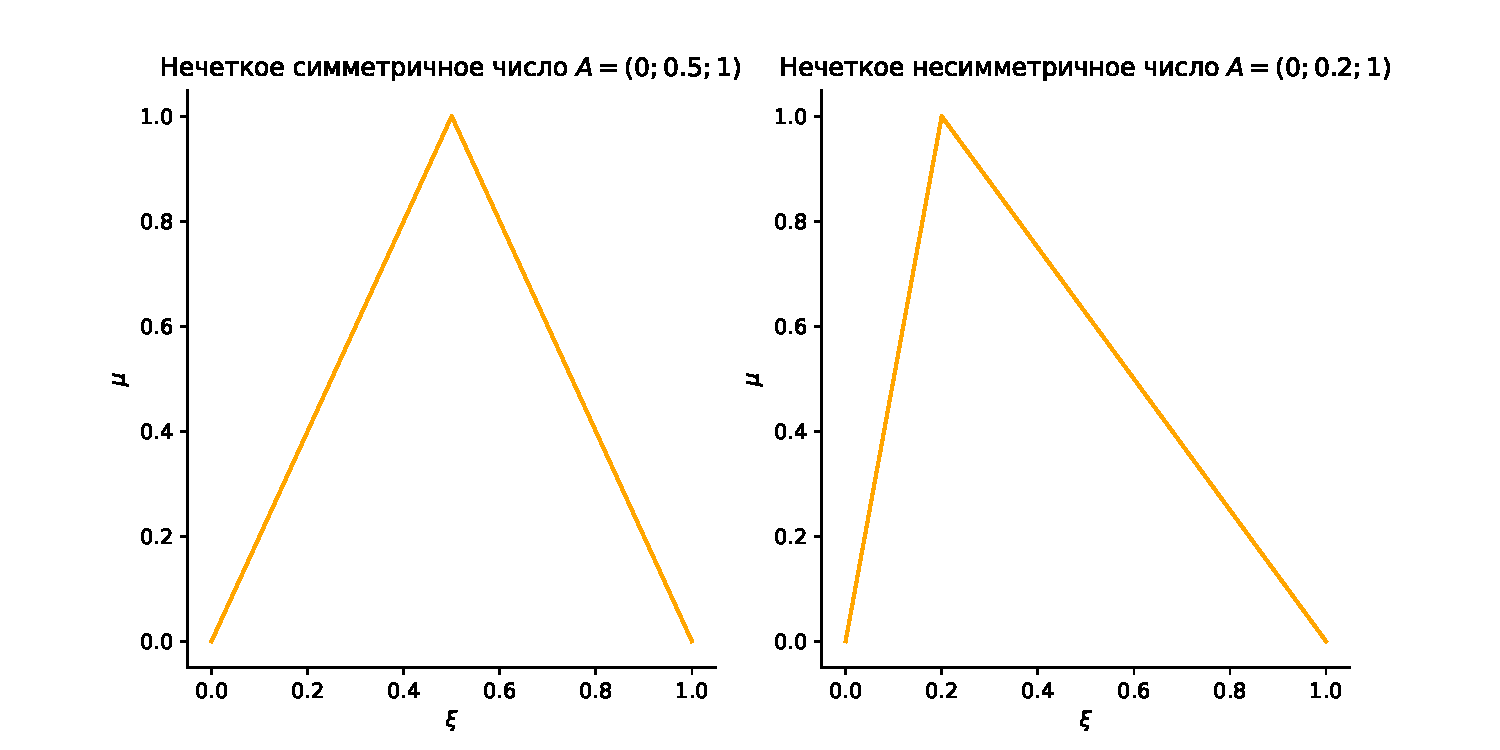
\includegraphics[width=\textwidth]{_images/Биномиальная модель на нечетких числах_1.pdf}
	\end{figure}
	
	Аналитически функцию принадлежности можно задать как \[\mu_A(x)=\begin{cases} \mu_{A_1}(\xi) \text{ , если } \xi \in [\xi_l;\xi_m) \\ \mu_{A_2}(\xi) \text{ , если } \xi \in [\xi_m;\xi_r) \\ 0 \text{ , иначе} \\ \end{cases}\] 
	
	(при условии, что максимум $\mu_A$ равен $1$ и достигается в точке $\xi = \xi_m$)
	
	Также заметим, что треугольное нечеткое число удобно представить в виде трехмерного вектора вида $(\xi_l;\xi_m;\xi_r)$, где числа $\xi_l$ и $\xi_r$ $-$ наибольшая и наименьшая границы $\mu$ $-$ среза числа $A$ при $\mu=0$, а число $\xi_m$ $-$ единственная точка $\mu$ среза числа $A$ при $\mu=1$. В случае использования такого подхода к заданию нечеткого числа удобно использовать такой переход \cite{6} от функции нечеткого числа к вектору $(\xi_l;\xi_m;\xi_r)$: если $\mu(\xi)=(\xi_l;\xi_m;\xi_r)$, то \[\mu_{\xi}=\begin{cases} \frac{\xi-\xi_l}{\xi_m-\xi_l} \text{, при } \xi \in [\xi_l;\xi_m) \\ \frac{\xi_r-\xi}{\xi_r-\xi_m} \text{, при } \xi \in [\xi_m;\xi_r) \\ 0 \text{, иначе } \end{cases}\]
	
	\section{Биномиальная модель для оценки опционов}
	Рассмотрим предпосылки, общепринятые обозначения, а также непосредственно теоретическую реализацию биномиальной модели как на действительных, так и на нечетких числах. 
	\subsection{Предпосылки}
	Введем предпосылки для биномиальной модели, в рамках которых мы будем работать в будущем:
	\begin{itemize}
		\item Нет арбитража
		\item Наличие постоянной безрисковой процентной ставки
		\item Бесконечная делимость ценных бумаг
		\item Отсутствие трансакционных издержек, налогов и комиссии
		\item Предположения относительно нормальности распределения цены базисного актива
		\item Постоянная волатильность базисного актива в течение срока действия опциона
		\item Коэффициент роста стоимости базисного актива обратно пропорционален коэффициенту понижению стоимости базисного актива
		\item Коэффициенты роста и понижения не изменяются в течение срока действия опциона $\Rightarrow$ модель будет давать осмысленный результат только при стабильно низкой волатильности акции
	\end{itemize}
	\subsection{Обозначения}
	Введем обозначения для параметров биномиальной модели:
	\begin{center}
		\begin{tabular}{|c|l|}
			\hline
			\textbf{Символ} & \textbf{Значение} \\
			\hline
			$C$ & цена опциона колл \\
			$P$ & цена опциона пут \\	
			$S$ & цена актива, на который покупается опцион \\
			$X$ & цена исполнения актива в конце срока его действия (страйк) \\
			$r$ & безрисковая процентная ставка \\
			$t$ & общее время действия опциона \\
			$\sigma$ & волатильность доходности базисного актива \\
			$N$ & количество шагов в биномиальной модели \\
			$dt$ & $\frac{t}{N}$ $-$ число разбиений в биномиальной модели \\
			\hline
		\end{tabular}
	\end{center}
	
	\subsection{Классическая биномиальная модель}
	Для расчета цены европейского опциона колл $C$ по биномиальной модели необходимо составить дерево всевозможных изменений цен базисного актива, на который покупается опцион и с учетом риск-нейтральной вероятности $p$ повышения цены актива на каждом шаге найти оптимальную цену опциона $C$. Коэффициенты повышения и понижения цены актива: $u=e^{\sigma \sqrt{dt}}$ и $d=\frac{1}{u}$ ($dt = \frac{t}{N}$). Риск-нейтральная вероятность $p$ определяется как $p=\frac{e^{r dt}-d}{u-d}$. Затем нужно рассчитать дерево всевозможных цен базисного актива. На первом шаге берется текущая цена актива; на втором шаге возможны цены $S \cdot u$ и $S \cdot d$; на третьем шаге возможны цены $S \cdot uu$, $S \cdot du=S \cdot ud$ и $S \cdot dd$. После этого необходимо инициализировать дерево цен опционов на базисный актив с последнего шага и прийти к финальной цене опциона. На каждом узле $i$ последнего шага дерева берем цену $\max{(S_i-X, 0)}$. Затем с переходим к предыдущему шагу дерева посредством рассчета математического ожидания соседних цен следующего шага: $p \cdot S_{j} + (1-p) \cdot S_{j+1}$. По такому алгоритму необходимо прийти к финальной цене опциона. 
	
	Продемонстрируем работу обычной биномиальной модели на действительных числах. В качестве примера рассчитаем биномиальную модель со следующими параметрами:
	\begin{center}
		\begin{tabular}{|c|l|}
			\hline
			\textbf{Параметр модели} & \textbf{Значение} \\
			\hline
			$S$ & $10$ \\
			$X$ & $10$ \\
			$t$ & $3$ \\
			$N$ & $10$ \\
			$r$ & $0.1$ \\
			$\sigma$ & $0.2$ \\
			\hline
		\end{tabular}
	\end{center}
	
	Рассчитаем $dt$: $dt = \frac{t}{N}=\frac{3}{10}=0.3$; $u=e^{\sigma \cdot \sqrt{dt}}=e^{0.2 \cdot \sqrt{0.3}}=1.116$ и $d=\frac{1}{u}=0.896$; $p=\frac{e^{r \cdot dt}-d}{u-d}=\frac{e^{0.1 \cdot 0.3}-0.896}{1.116-0.896}=0.611$. Если выполнить алгоритм биномиальной модели с $N=10$, то получим $C=2.873$
	
	\subsection{Биномиальная модель на нечетких числах}
	При реализации биномиальной модели на нечетких числах попробуем работать не с функцией принадлежности непосредственно, а с вектором вида $(\xi_l;\xi_m;\xi_r)$ для треугольного нечеткого числа. При этом мы будем работать с каждым элементом этого вектора как с обычным числом, применяя к нем обычные математические функции. В таком случае также возникают проблемы, связанные с тем, что полученный результат может не быть нечетким числом в соответствие с заданным определением. По этой причине предлагается применять некоторые преобразования для вектора $(\xi_l;\xi_m;\xi_r)$. В частности, к вектору $(\xi_l;\xi_m;\xi_r)$ будем применять только строго монотонные преобразования (при этом если применяемая к вектору функция убывает, то поменяем крайние элементы вектора местами). Таким образом, полученное в качестве цены опциона нечеткое число по сути будет представлять собой значение цены опциона, рассчитанной с помощью обычной биномиальной модели на действительных числах в самом лучшем случае, в обычном случае, в лучшем случае. Именно поэтому необходимо обращать внимание не только на срезы этого нечеткого числа при $\mu=1$ или $\mu=0$. 
	
	Пусть для биномиальной модели заданы следующие параметры: $S, X, N=2, t$ как обычные числа, а $r$ и $\sigma$ $-$ как нечеткие числа $(r_l;r_m;r_r)$ и $(\sigma_l;\sigma_m;\sigma_r)$ соответственно. Найдем цену опциона по биномиальной модели. Рассчитаем $u$: 
	$u=e^{(\sigma_l;\sigma_m;\sigma_r) \cdot \sqrt{dt}} = (e^{\sqrt{dt} \cdot \sigma_l};e^{\sqrt{dt} \cdot \sigma_m};e^{\sqrt{dt} \cdot \sigma_r})$ (при $dt=\frac{t}{N}$); 
	$d=\frac{1}{u}=\frac{(1;1;1)}{(e^{\sqrt{dt} \cdot \sigma_l};e^{\sqrt{dt} \cdot \sigma_m};e^{\sqrt{dt} \cdot \sigma_r})}=(\frac{1}{e^{\sqrt{dt} \cdot \sigma_r}};\frac{1}{e^{\sqrt{dt} \cdot \sigma_m}};\frac{1}{e^{\sqrt{dt} \cdot \sigma_l}})$. 
	
	Теперь рассчитаем риск-нейтральную вероятность \[p=\frac{e^{r \cdot dt}-d}{u-d}=\frac{e^{(dt \cdot r_l;dt \cdot r_m;dt \cdot r_r)}-\left(\frac{1}{e^{\sqrt{dt} \cdot \sigma_r}};\frac{1}{e^{\sqrt{dt} \cdot \sigma_m}};\frac{1}{e^{\sqrt{dt} \cdot \sigma_l}}\right)}{(e^{\sqrt{dt} \cdot \sigma_l};e^{\sqrt{dt} \cdot \sigma_m};e^{\sqrt{dt} \cdot \sigma_r})-\left(\frac{1}{e^{\sqrt{dt} \cdot \sigma_r}};\frac{1}{e^{\sqrt{dt} \cdot \sigma_m}};\frac{1}{e^{\sqrt{dt} \cdot \sigma_l}}\right)}\].
	
	Теперь можно построить дерево со всевозможными ценами ценами базисного актива (например, акции). Поскольку число шагов $N=2$, то в дереве будет $3$ шага с соответственно $1$, $2$, $3$ возможными ценами актива:
	
	\begin{figure}[H]
		\centering
		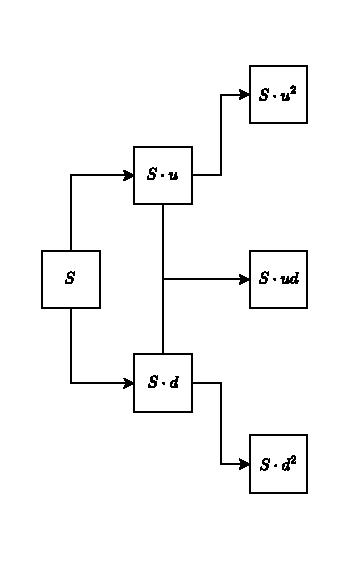
\includegraphics[width=0.4\textwidth]{_images/Биномиальная модель на нечетких числах_1.drawio.pdf}
	\end{figure}
	
	Теперь можно пройтись по дереву с конца и рассчитать нечеткую стоимость опциона: 
	
	\begin{figure}[H]
		\centering
		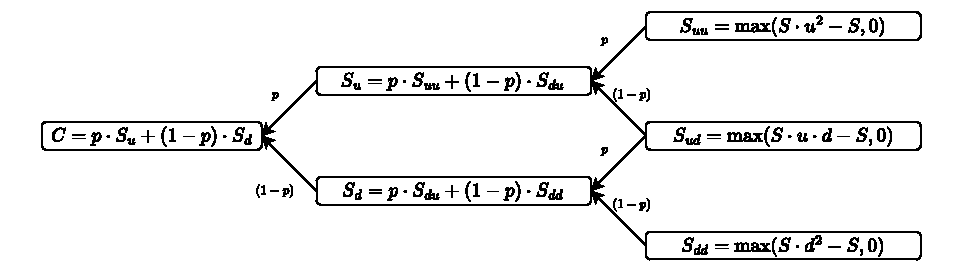
\includegraphics[width=\textwidth]{_images/Биномиальная модель на нечетких числах_2.drawio.pdf}
	\end{figure}
	
	Таким образом, мы нашли нечеткую цену для европейского опциона колл: 
	
	\begin{equation}
		\begin{split}
			C=p\cdot[p \cdot \max(S \cdot u^2 - S, 0) + (1-p) \cdot \max(S \cdot ud - S, 0)]
			\\
			+(1-p)\cdot[p \cdot \max(S \cdot ud - S, 0) + (1-p)\cdot \max(S\cdot d^2-S, 0)]
		\end{split}
	\end{equation}
	
	Продемонстрируем на конкретном примере работу данного подхода к биномиальной модели на нечетких числах:
	
	\begin{center}
		\begin{tabular}{|c|l|}
			\hline
			\textbf{Параметр модели} & \textbf{Значение} \\
			\hline
			$S$ & $(100, 100, 100)$ \\
			$X$ & $105$ \\
			$t$ & $1$ \\
			$N$ & $2$ \\
			$r$ & $(0.08; 0.1; 0.12)$ \\
			$\sigma$ & $(0.18; 0.2; 0.22)$ \\
			\hline
		\end{tabular}
	\end{center}
	
	По выведенной для $C$ формуле можно посчитать, что $C=(11.603,13.566,14.601)$ (с точностью до тысячных). Заметим, что число $13.566$ $-$ цена опциона по обычной модели $-$ не является серединой отрезка цен $\frac{11.603+14.601}{2}$. Это свидетельствует о том, что при оценке некоторого опциона можно ориентироваться не только на срез $\mu=1$, то также и на срезы для $\mu: \mu < 1$ $-$ в этом и состоит идея оценки опциона нечетких числом. 
	
	\begin{figure}[H]
		\centering
		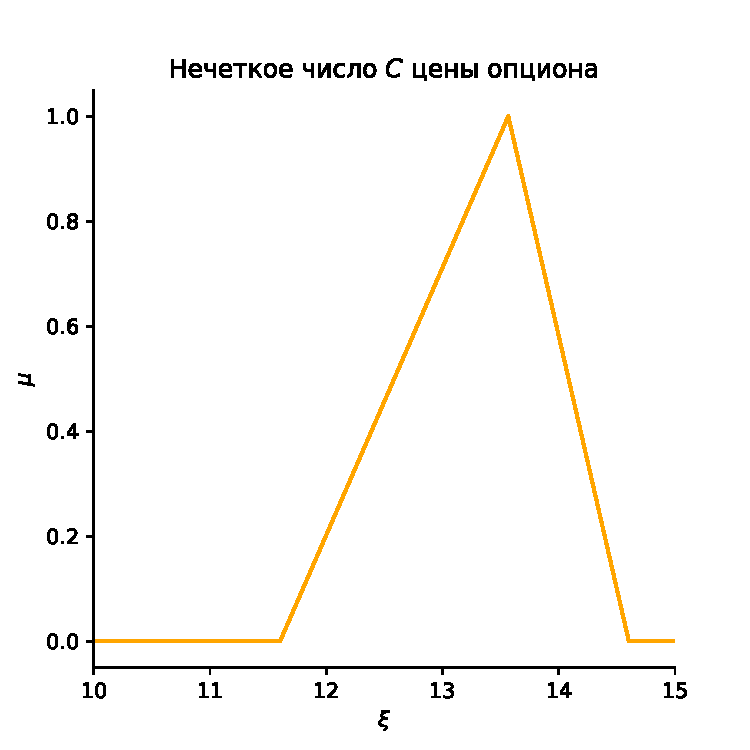
\includegraphics[width=0.5\textwidth]{_images/Биномиальная модель на нечетких числах_3.pdf}
	\end{figure}
	
	\section{Проблемы биномиальной модели на нечетких числах}
	Было замечено, что при расчете биномиальной модели с достаточно большим $N$ $(N \to \infty)$ происходит "разъезжание" левой и правой границ нечеткого числа, вследствие чего получается, что для нечеткого числа цены опциона $(\xi_l, \xi_m, \xi_r)$ при $N \to \infty$ будет $\xi_l \to 0$ и $\xi \to +\infty$. Такой результат приводит к неразумности использования биномиальной модели на нечетких числах при $N \to \infty$, поскольку при высокой вычислительной сложности биномиальная модель на нечетких числах не давает осмысленный результат, отличающийся от обычной биномиальной модели на действительных числах. Покажем это: пусть есть некоторые параметры для оценки стоимости опциона, содержащие нечеткие числа:
	\begin{center}
		\begin{tabular}{|c|l|}
			\hline
			\textbf{Параметр модели} & \textbf{Значение} \\
			\hline
			$S$ & $(9, 10, 11)$ \\
			$X$ & $10$ \\
			$t$ & $3$ \\
			$r$ & $(0.05; 0.1; 0.15)$ \\
			$\sigma$ & $(0.1; 0.2; 0.3)$ \\
			$N$ & $5$ \\
			\hline
		\end{tabular}
	\end{center}
	
	С такими параметрами получаем цену европеского опциона колл $C=(0.089, 2.913, 11.305)$ $\Rightarrow$ срез нечеткого числа при $\mu=1$: $[0.089, 11.305]$. Можно отметить, что срез слишком большой и не дает осмысленного результата.
	\begin{figure}[H]
		\centering
		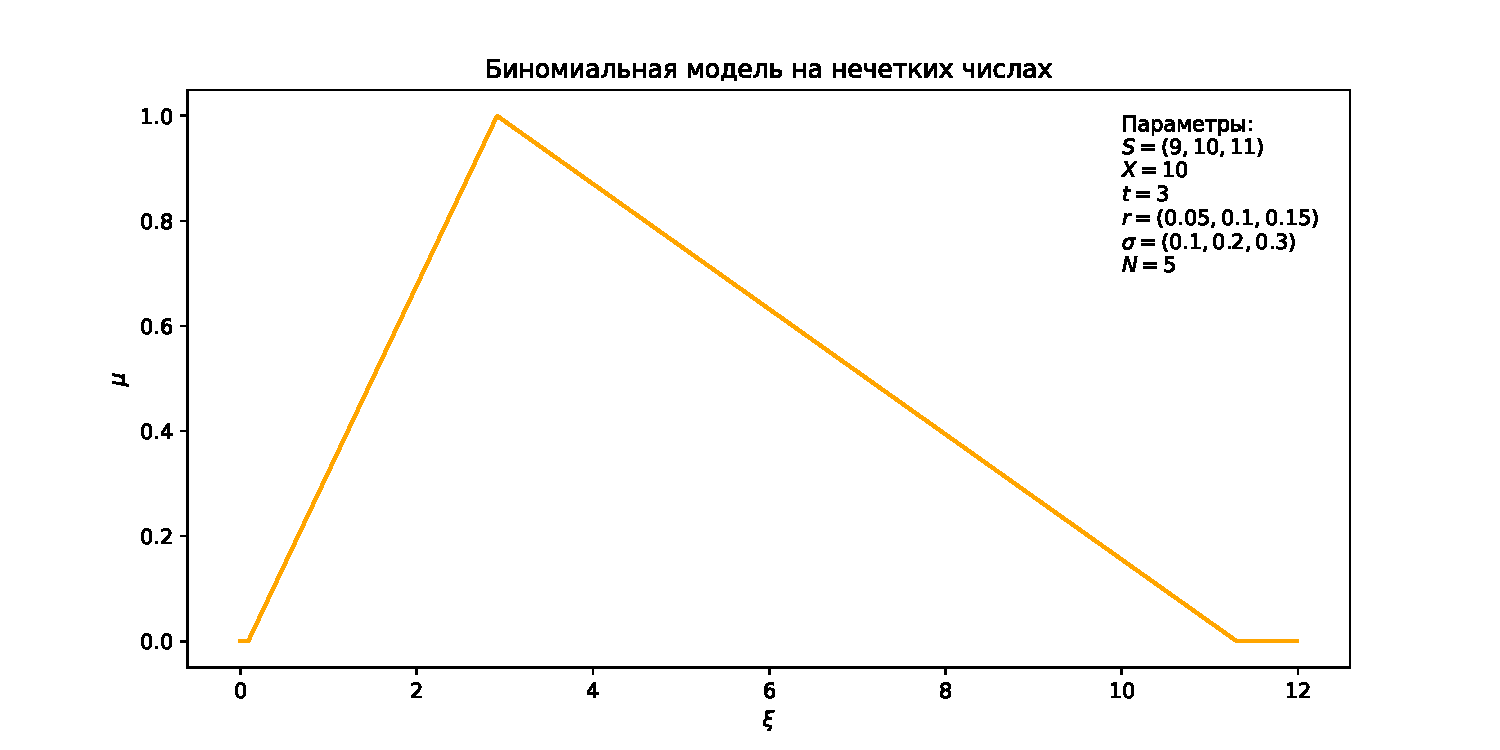
\includegraphics[width=0.8\textwidth]{_images/fuzzy-binomial.pdf}
	\end{figure}
	
	Рассчитаем теперь модель Блэка-Шоулза на нечетких числах с такими же параметрами. Очевидно, что мы получим средний индекс нечеткого числа стоимости опциона $C$ близкий по значению к $2.913$ (из-за сходимости биномиальной модели к модели Блэка-Шоулза при $N \to \infty$ \cite{1}); однако левый и правый индекс $C$ по Блэку-Шоулзу будут существенно отличаться от левого и правого индексов по биномиальной модели: $C=(0.824, 2.907, 4.946)$ $-$ более разумный результат и срез при $C$ при $\mu=1$ будет равен $(0.824, 4.946)$. 
	\begin{figure}[H]
		\centering
		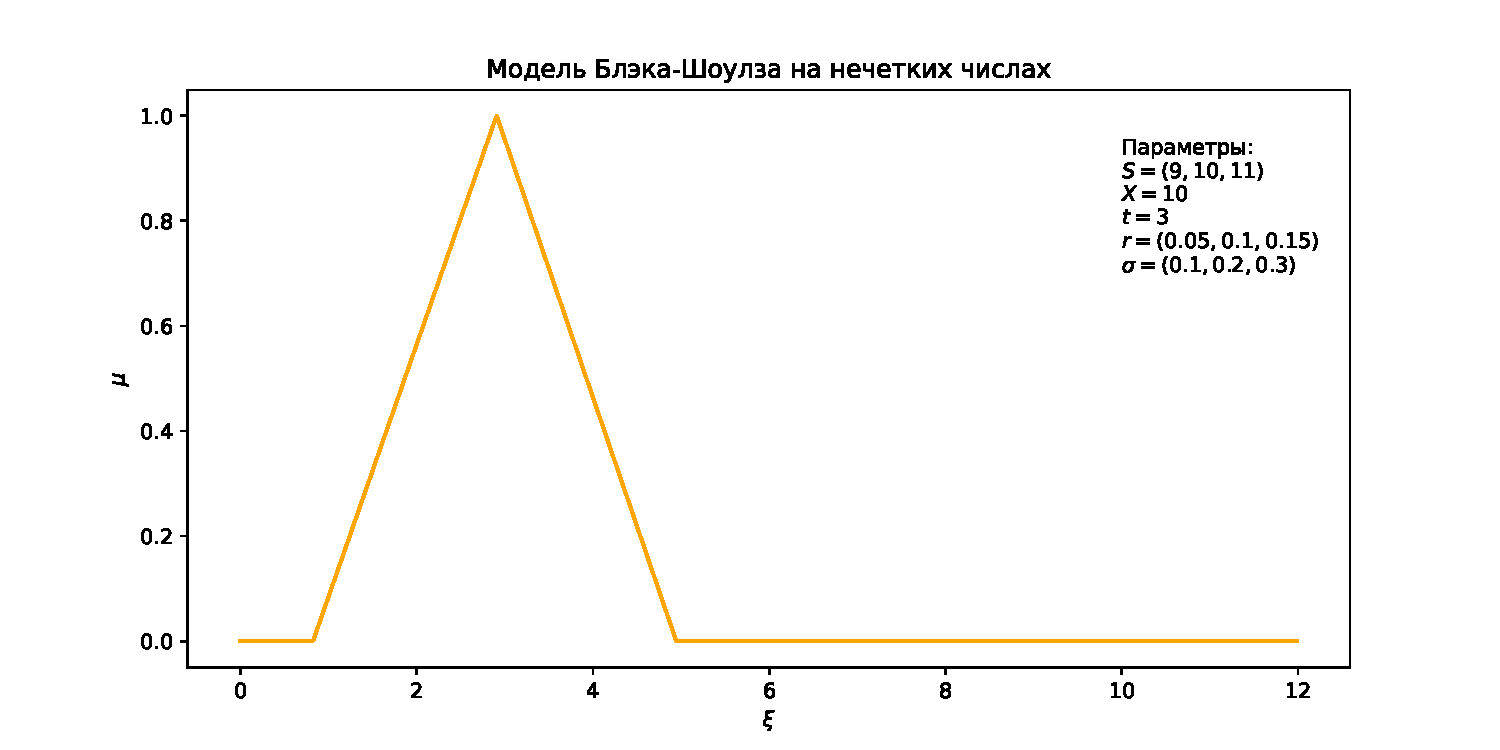
\includegraphics[width=\textwidth]{_images/fuzzy-black-scholes.pdf}
	\end{figure}
	
	Из графиков видно, что уже при $N=5$ биномиальная модель дает результат, левый индекс которого почти нулевой, а правый индекс $-$ слишком большой. Продемонстрируем, как меняются эти индексы при $N \to \infty$. Левый индекс:
	\begin{figure}[H]
		\centering
		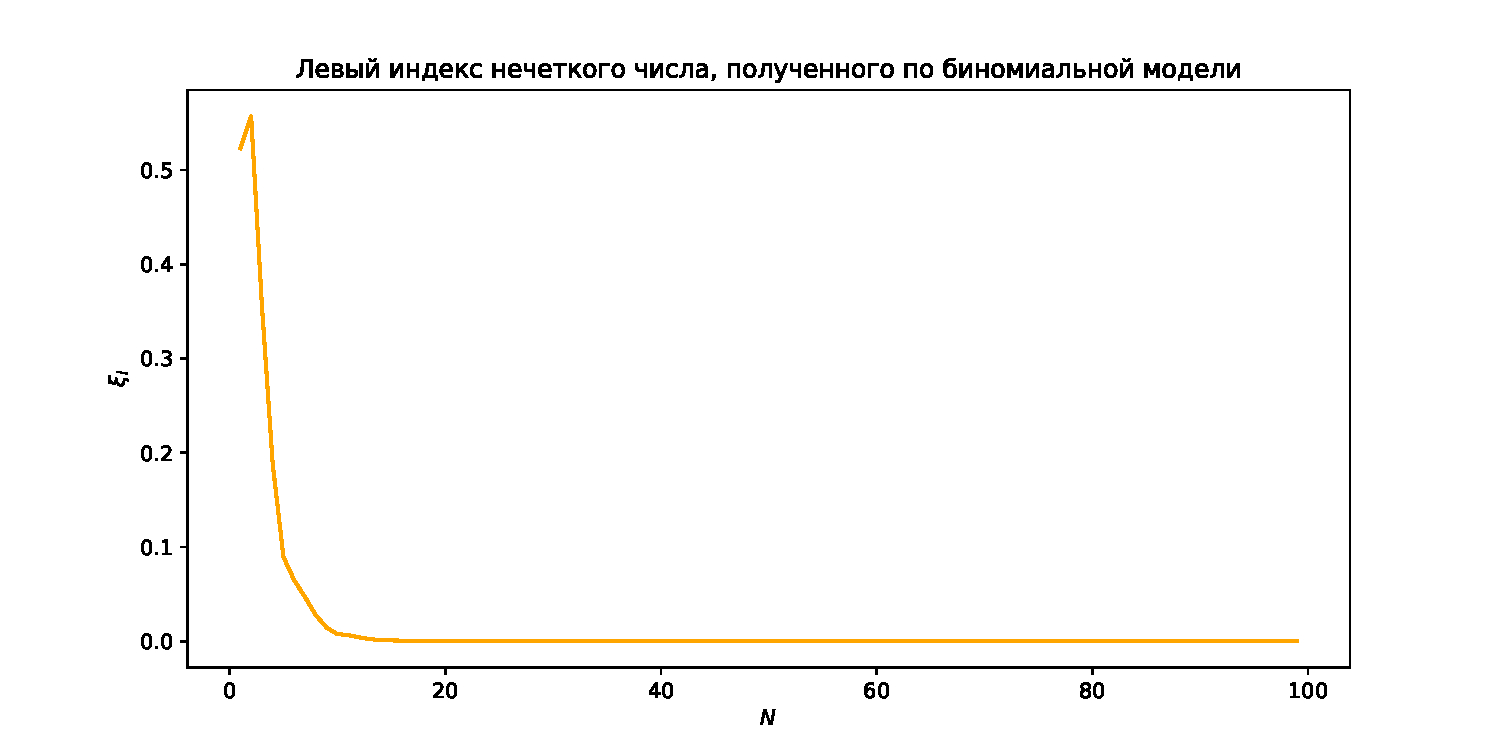
\includegraphics[width=\textwidth]{_images/left-fuzzy-binomial.pdf}
	\end{figure}
	
	Средний индекс:
	\begin{figure}[H]
		\centering
		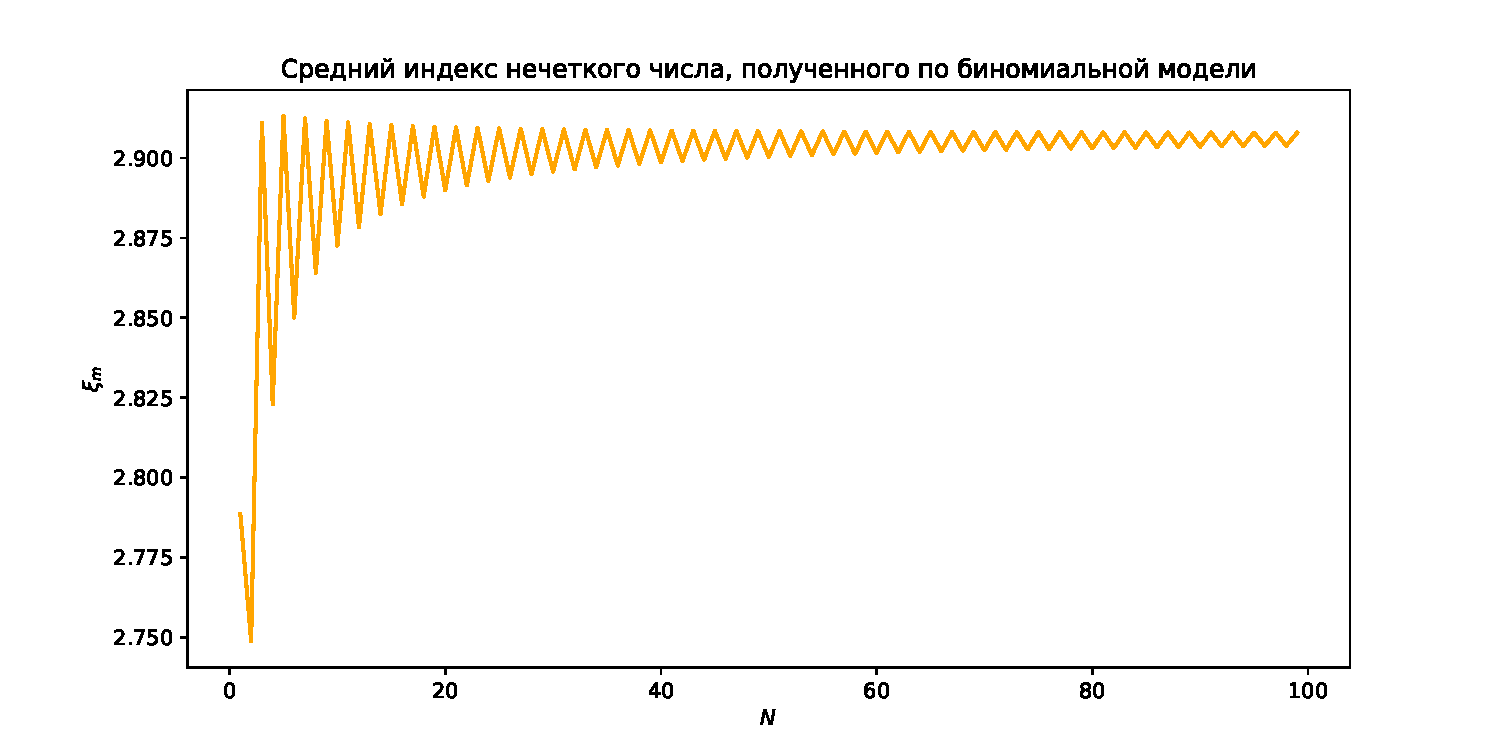
\includegraphics[width=\textwidth]{_images/middle-fuzzy-binomial.pdf}
	\end{figure}
	
	Правый индекс:
	\begin{figure}[H]
		\centering
		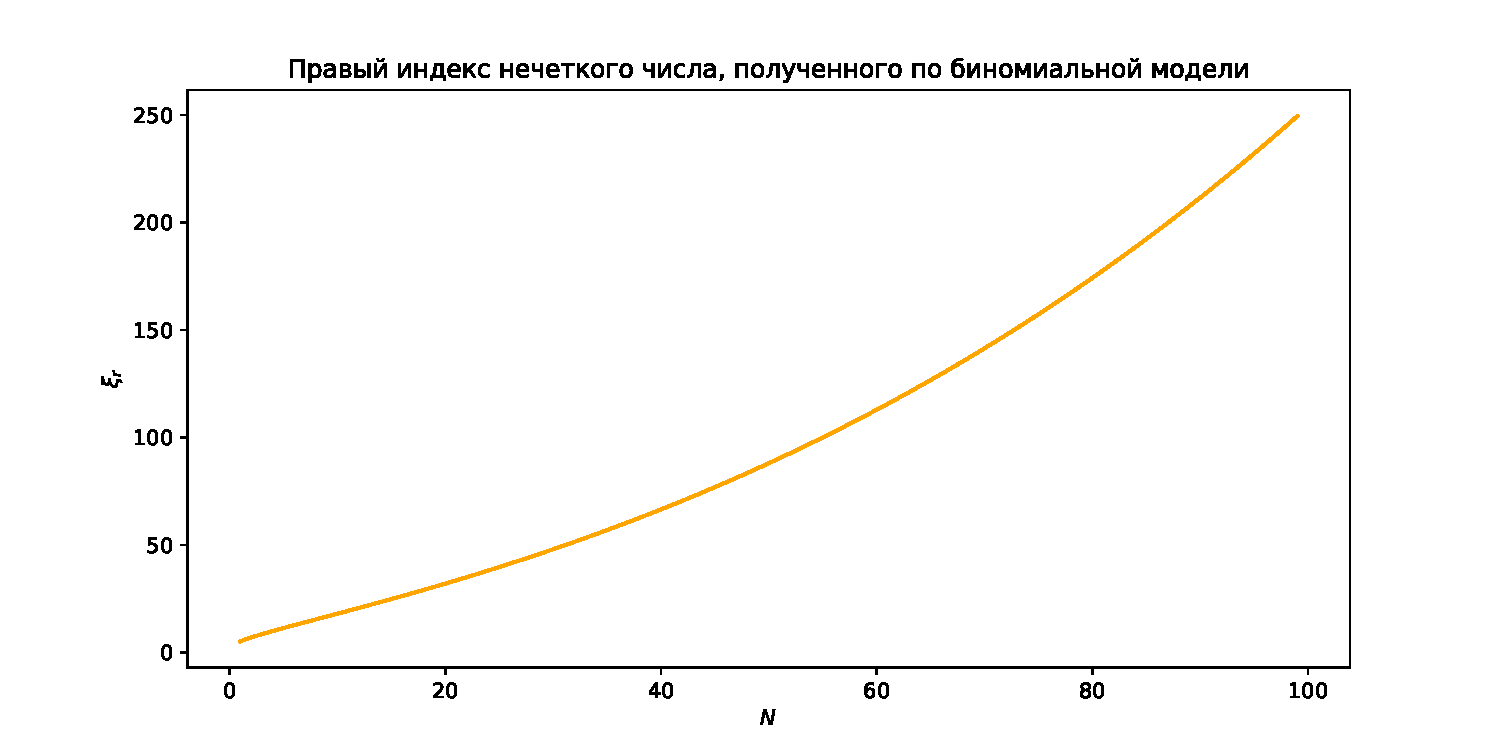
\includegraphics[width=\textwidth]{_images/right-fuzzy-binomial.pdf}
	\end{figure}
	
	Сходимость биномиальной модели к модели Блэка-Шоулза по среднему индексу нечеткого числа $C$:
	\begin{figure}[H]
		\centering
		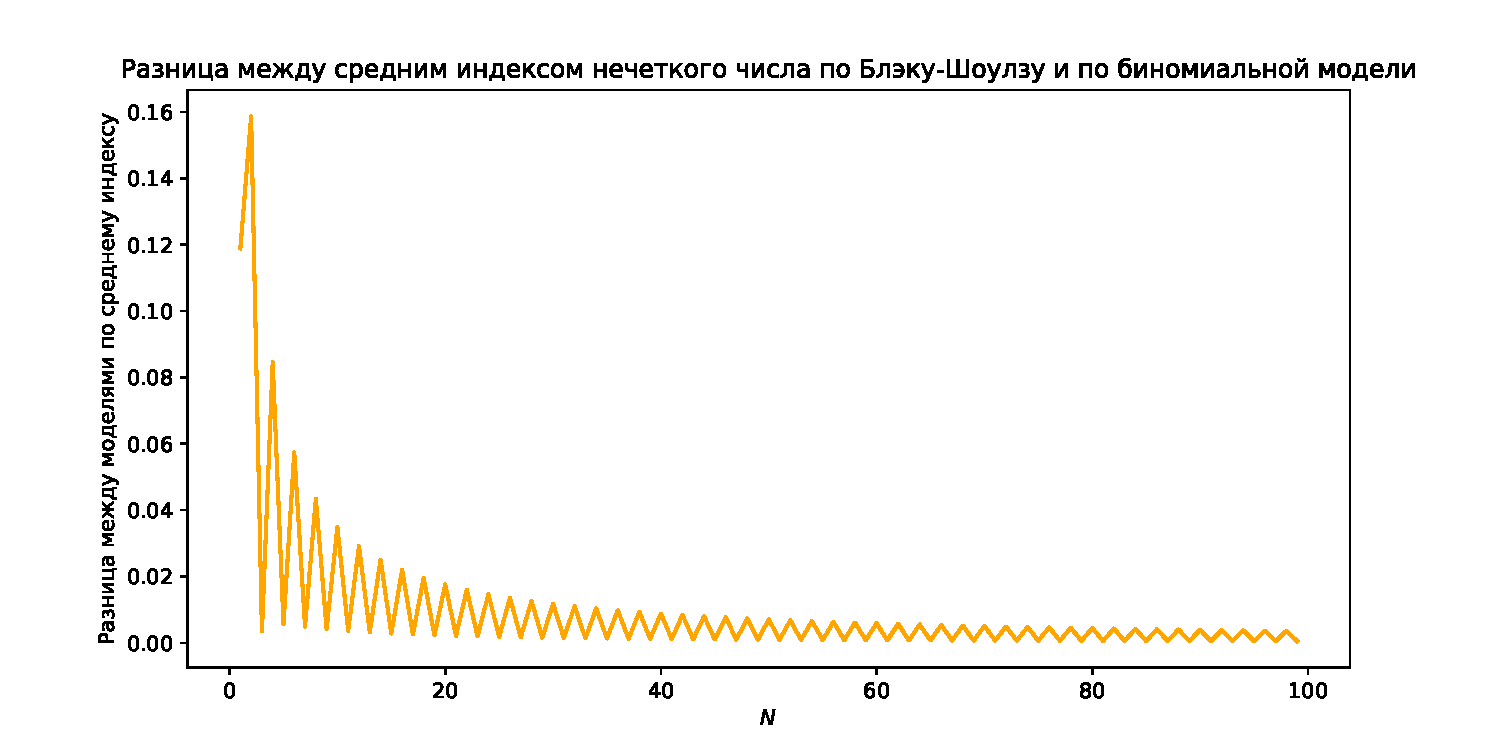
\includegraphics[width=\textwidth]{_images/middle-fuzzy-binomial-to-middle-fuzzy-black-scholes.pdf}
	\end{figure}
	
	Таким образом, из графиков видно, что при $N \to \infty$ будет $\xi_l \to 0$ и $\xi_r \to \infty$. Этот результат можно объяснить тем, что при $N \to \infty$ левый индекс нечеткого числа $C$ будет показывать цену опциона при самой худшей ситуации (с минимальной волатильностью $\sigma$ , минимальной процентной ставкой $r$ и минимальной текущей ценой базисного актива $S$ при постоянном понижении цены базисного актива) $\Rightarrow$ такая цена будет стремиться к $0$ при увеличении числа шагов; в то время, как самый лучший исход биномиальной модели будет очень большим. Оба этих события маловероятны, и поэтому необходимо каким-либо образом дефаззифицировать нечеткое число $C$, чтобы получать меньший срез при $\mu=1$. При этом чем больше в модели нечетких входных параметров, тем быстрее "расходится" ее результат при $N \to \infty$. Поэтому мы будем использовать биномиальную модель, где нечеткой будет только волатильность. 	
	
	\section{Обзор литературы по биномиальной модели на нечетких числах}
	Для того, чтобы решить проблему с <<разъезжанием>> нечеткого числа при использовании биномиальной модели, рассмотрим реализацию биномиальной модели на нечетких числах у других авторов. Всего рассмотрим $2$ статьи:
	\begin{itemize}
		\item <<Model construction of option pricing based on fuzzy theory>> \cite{2} (Shang-En Yu, Ming-Yuan Leon Li, Kun-Huang Huarng, Tsung-Hao Chen, and Chen-Yuan Chen)
		\item <<A Fuzzy Set Approach for Generalized CRR Model: An Empirical Analysis of S\&P 500 Index Options>> \cite{3} (Cheng Few Lee, Gwo-Hshiungtzeng, Shin-Yun Wang)
	\end{itemize}
	\subsection{Обзор статьи <<A Fuzzy Set Approach for Generalized CRR Model: An Empirical Analysis of S\&P 500 Index Options>>}
	Обзор статьи <<A Fuzzy Set Approach for Generalized CRR Model: An Empirical Analysis of S\&P 500 Index Options>> \cite{3} (Cheng Few Lee, Gwo-Hshiungtzeng, Shin-Yun Wang). Главная модификация биномиальной модели, представленная авторами в данной статье, состоит в том, что рассматриваются 6 чисел, задающих различное изменение цен: $(u_l, u_m, u_r)$ и $(d_l, d_m, d_r)$ $-$ слабое, средние и сильное повышение цены на базисный актив. На каждом шаге стоимость базисного актива может подняться до $S_{ur}=S\cdot[e^{(1+r)\sigma \sqrt{dt}}],S_{um}=S\cdot[e^{\sigma \sqrt{dt}}],S_{ul}=S\cdot[e^{(1-r)\sigma \sqrt{dt}}]$ и опуститься до $S_{dr}=S\cdot[e^{-(1-r)\sigma \sqrt{dt}}],S_{dm}=S\cdot[e^{-\sigma \sqrt{dt}}],S={dl}=S\cdot[e^{-(1+r)\sigma \sqrt{dt}}]$. Цены опционов колл $C_{ur} = \max(S_{ur} - X,0)$, $C_{um} = \max(S_{um} - X,0)$, $C_{ul} =
	\max(S_{ul} - X,0)$, $C_{dr} = \max(S_{dr} - X,0)$, $C_{dm} = \max(S_{dm} - X,0)$, $C_{dl} = \max(S_{dl} - X,0)$. Также задается $3$ риск-нейтральные вероятности: $p_{u}=\frac{e^{r_h dt - d_l}}{u_r-d_l}$, $p_m=\frac{e^{r_m dt}-d_m}{u_m-d_m}$, $p_d=\frac{e^{r_l\Delta t}-d_r}{u_l-d_r}$. Таким образом, авторы получают такую нечеткую цену европейского опциона колл для двухшаговой биномиальной модели: $C=\begin{cases} C_u=e^{-r_l dt}[p_u\cdot C_{ur}+(1-p)\cdot C_{dl}] \\ C_m=e^{-r_m dt}[p_m\cdot C_{ur}+(1-p_m)\cdot C_{dl}] \\ C_d=e^{-r_h dt}[p_d\cdot C_{ul} + (1-p_d)\cdot C_{dr}]) \\ \end{cases}$
	
	\subsection{Обзор статьи <<Model construction of option pricing based on fuzzy theory>>}
	Обзор статьи <<Model construction of option pricing based on fuzzy theory>> \cite{2} (Shang-En Yu, Ming-Yuan Leon Li, Kun-Huang Huarng, Tsung-Hao Chen, and Chen-Yuan Chen). Авторы статьи используют принцип, аналогичный использованному в \cite{3}. Таким образом, строится дерево с $6^{n-1}$ вершинами на последнем шаге $n$ и производится обратный проход с конца дерева стоимостей опционов до начала дерева. Авторы, исследуя реальные данные о ценах опционах, приходят к выводу, что точность прогноза такой биномиальной модели оказывается выше в сравнении с классической моделью. При этом левый индекс нечеткой цены опциона $C$ предлагается использовать несклонным к риску агентам, а правый индекс $-$ склонным к риску агентам.
	
	\section{Возможные решения проблем биномиальной модели на нечетких числах}
	В этом разделе рассмотрим, как можно решить проблему "разъезжания" левого и правого индексов нечеткого числа $-$ цены опциона так, чтобы при $N \to \infty$ результат модели асимптотически сходился к некоторому конкретному значению по всем индексам, а не "расходился". Всего было предложено $3$ метода, из которых действенным оказался последний $-$ с нормировкой волатильности. 
	
	\subsection{Нормировка стоимостей базисного актива}
	Было проверено, что при расчете нечеткой биномиальной модели проблема 
	$\begin{cases}
		\xi_l \to 0 \\
		\xi_r \to \infty \\
	\end{cases}$ 
	проявляется уже на этапе рассчета возможных стоимостей бизисного актива: минимальная возможная цена базисного актива при больших $N$ стремится к нулю , а максимальная возможная цена базисного актива $-$ к бесконечности. Поэтому было решено нормировать нечеткие цены базисного актива. Для этого при расчете каждой возможной цены актива в качестве левого коэффициента мы брали $S_l = S_m - S_l \cdot \alpha$, а в качестве правого $-$ $S_r = S_m + S_r \cdot \alpha$, где $\alpha$ $-$ некоторый экзогенный параметр, который можно интерпретировать, как степень расплывчатости стоимости актива. При таком подходе средний индекс результата модели все еще будет сходится к формуле Блэка-Шоулза по центральному индексу, однако непонятно, каким нужно выбрать $\alpha$, чтобы нечеткая биномиальная модель выдавала стоимость опциона, не зависящую от числа шагов $N$. При следующих входных параметрах:
	 \begin{center}
	 	\begin{tabular}{|c|l|}
	 		\hline
	 		\textbf{Параметр модели} & \textbf{Значение} \\
	 		\hline
	 		$S$ & $1$ \\
	 		$X$ & $1$ \\
	 		$t$ & $1$ \\
	 		$r$ & $0.1$ \\
	 		$\sigma$ & $(0.1; 0.12; 0.15)$ \\
	 		$N$ & $100$ \\
	 		$\alpha$ & $0.5$ \\
	 		\hline
	 	\end{tabular}
	 \end{center}
	 
	 результат модели $-$ нечеткое число $[0, 0.1079, 1.1853]$, которое также "расходится". 
	 
	\subsection{Сужение массива цен базисного актива}
	Поэтому было решено использовать не все возможные цены базисного актива для построения дерева цен опциона, а только долю $\alpha \in (0,1)$ средних цен активов. При таком подходе модель не учитывает самые лучшие и самые худшие сценарии для изменения цен базисного актива, что приводит к усреднению ее результатов. Однако такая модификация биномиальной модели приводит к появлению дополнительного гиперпараметра, который нужно как-то подбирать. Для тестов было использовано $\alpha=\min(\sigma_m; 1)$, так как при росте волатильности и неопределенности логичнее рассматривать большую часть от стоимостей актива. Кроме того, из-за того, что массив цен актива модифицируется, то центральный индекс нечеткого результата не будет гарантированно сходится к формуле Блэка-Шоулза. Были проведены тесты такой модификации модели на следующих параметрах: 
	\begin{center}
		\begin{tabular}{|c|l|}
			\hline
			\textbf{Параметр модели} & \textbf{Значение} \\
			\hline
			$S$ & $1$ \\
			$X$ & $1$ \\
			$t$ & $1$ \\
			$r$ & $0.1$ \\
			$\sigma$ & $(0.1; 0.12; 0.15)$ \\
			$N$ & $100$ \\
			\hline
		\end{tabular}
	\end{center}
	
	Результатом такой модели будет нечеткое число $[0, 0.1079, 0.3001]$, которое также не является разумным результатом. 
	
	\subsection{Нормировка волатильности}
	Поскольку "разъезжание" нечетких чисел происходит уже на этапе расчета стоимостей активов, то разумно нормировать волатильность сразу так, чтобы она уменьшалась при увеличении $N$. Возьмем волатильность $\sigma=(\sigma_l, \sigma_m, \sigma_r)=(\sigma_m - \frac{\sigma_l}{\sqrt{N}}, \sigma_m, \sigma_m + \frac{\sigma_r}{\sqrt{N}})$. С такой волатильностью модификация биномиальной модели будет сходиться к формуле Блэка-Шоулза по центральному индексу. Для тестов модели возьмем такие параметры: 
	\begin{center}
		\begin{tabular}{|c|l|}
			\hline
			\textbf{Параметр модели} & \textbf{Значение} \\
			\hline
			$S$ & $1$ \\
			$X$ & $1$ \\
			$t$ & $1$ \\
			$r$ & $0.1$ \\
			$\sigma$ & $(0.1; 0.12; 0.15)$ \\
			$N$ & $100$ \\
			\hline
		\end{tabular}
	\end{center}
	
	С заданными параметрами получаем цену опциона $[0.0294, 0.10795, 0.2434]$. Стоимость опциона не "разъезжается". Более того, при увеличении $N$ (было численно проверенно для $N$ до $3000$) такая модификация нечеткой биномиальной модели будет сходиться к конкретному нечеткому числу и не зависеть от $N$:
	
	\begin{figure}[H]
		\centering
		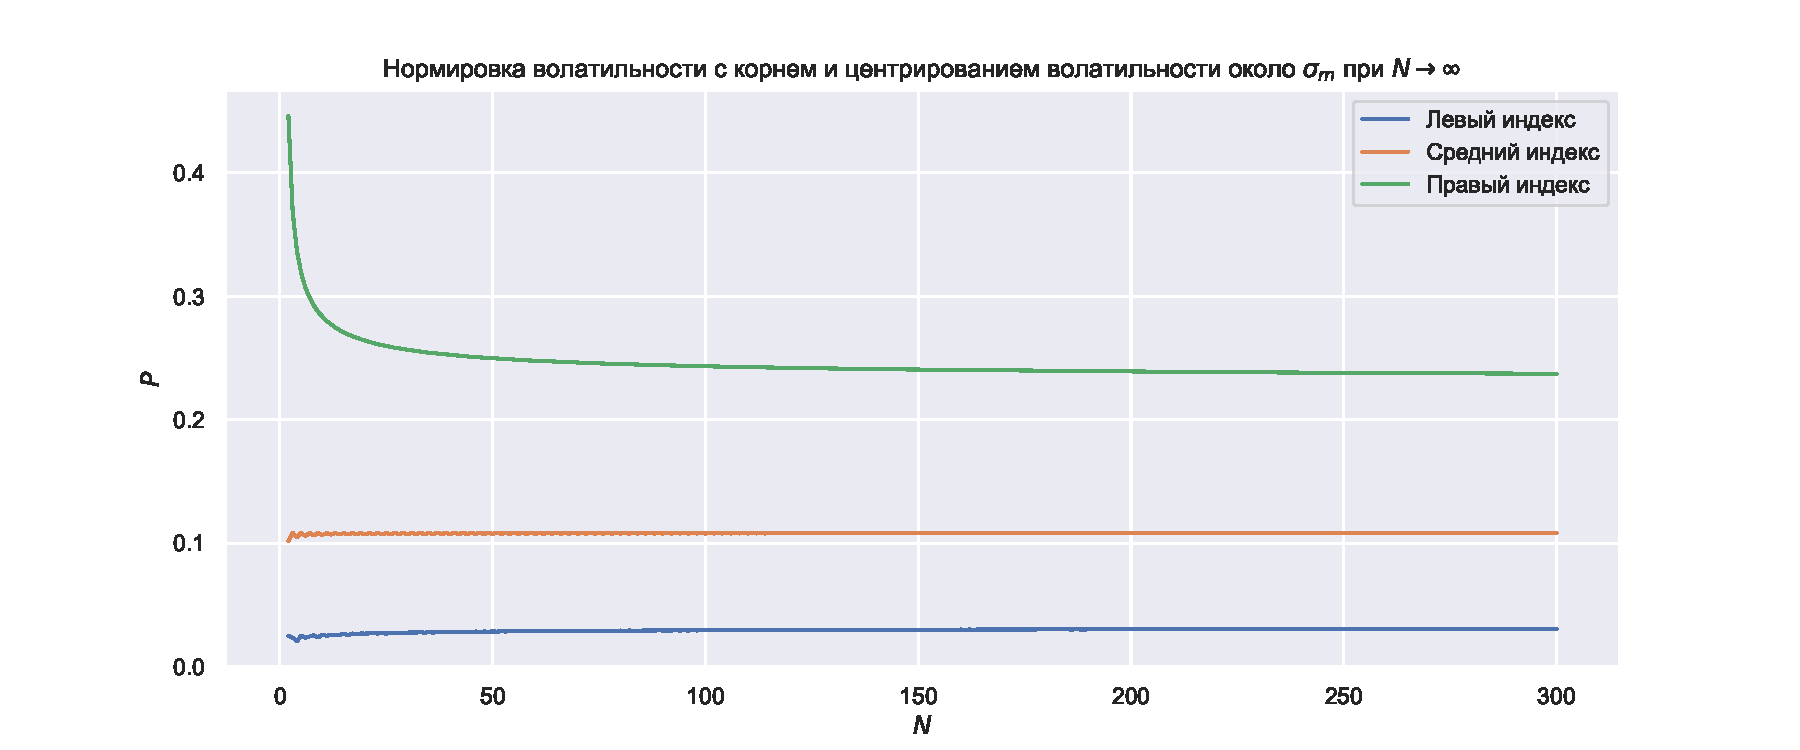
\includegraphics[width=\textwidth]{_images/Нормировка волатильности с корнем и центрированием волатильности около $sigma_m$.pdf}
	\end{figure}
	
	\section{Реализация и тесты в \textbf{python}}
	В \href{https://drive.google.com/file/d/1pRsXcyhmx7AT0D3hcHYBzhjENuwIqE97/view?usp=sharing}{приложении} с реализацией моделей в среде \textbf{python} есть функции для: 
	\begin{itemize}
	\item Классической модели Блэка-Шоулза
	\item Классической биномиальной модели
	\item Модели Блэка-Шоулза с нечеткими числами
	\item Биномиальной модели с нечеткими числами
	\item Нечеткой биномиальной модели с нормировкой стоимостей базисного актива
	\item Нечеткой биномиальной модели с уменьшением массива стоимостей базисного актива
	\item Нечеткой биномиальной модели с нормировкой волатильности с использованием разных функций (корня, логарифма и линейной)
	\end{itemize}
	
	\section{Выводы и результаты}
	\begin{itemize}
		\item Изучили и реализовали классическую биномиальную модель и модель Блэка-Шоулза
		\item Рассмотрели и реализовали нечеткие версии модели Блэка-Шоулза и биномиальной модели
		\item Выявили проблему биномиальной модели на нечетких числах
		\item Сделали обзор литературы по биномиальной модели на нечетких числах
		\item Предложили (без доказательства) модификацию нечеткой биномиальной модели, сходящуюся к конкретному нечеткому числу при $N \to \infty$
	\end{itemize}
	\newpage{}
	
	\begin{thebibliography}{99}
		\bibitem{1} S. Roman <<Introduction to the Mathematics of Finance>>
		\bibitem{2} Shang-En Yu, Ming-Yuan Leon Li, Kun-Huang Huarng, Tsung-Hao Chen, and Chen-Yuan Chen <<Model construction of option pricing based on fuzzy theory>>
		\bibitem{3} Cheng Few Lee, Gwo-Hshiungtzeng, Shin-Yun Wang <<A Fuzzy Set Approach for Generalized CRR Model: An Empirical Analysis of S\&P 500 Index Options>>
		\bibitem{4} Лис А. И. <<О применении нечетких чисел при оценке опционов>>
		\bibitem{5} Шведов А. С. <<О математических методах, используемых при работе с опционами>>
		\bibitem{6} A. Thavaneswaran, S. S. Appadoo, J. Frank <<Binary option pricing using fuzzy numbers>>
		\bibitem{7} Jorge de Andrés-Sánchez <<Modelling Up-and-Down Moves of Binomial Option Pricing with Intuitionistic Fuzzy Numbers>>
	\end{thebibliography}
	\newpage{}
	
	\tableofcontents{}
	
\end{document}
